Notre projet informatique intègre actuellement toutes les fonctionnalités prévues dans le cahier des charges. Nous avons donc atteint les objectifs fixés dans la présentation.\\

De plus, nous avons apporté des améliorations supplémentaires au projet par rapport au cahier des charges. Ces ajouts ont contribué à améliorer l'expérience utilisateur.\\

Nous avons, tout d'abord, amélioré la gestion des étudiants en permettant aux enseignant de supprimer les comptes des étudiants au cas par cas ou tous les étudiants en même temps, comme montré dans la figure \ref{fig:ajouts}.\\

Ensuite nous avons amélioré la gestion des étiquettes en permettant aux enseignants de modifier leurs étiquettes et de les supprimer comme le montre également la figure \ref{fig:ajouts}. Cet ajout permet d'offrir aux enseignants plus de flexibilité pour organiser leurs questions.\\

\vspace{2mm}
\begin{figure}[H]
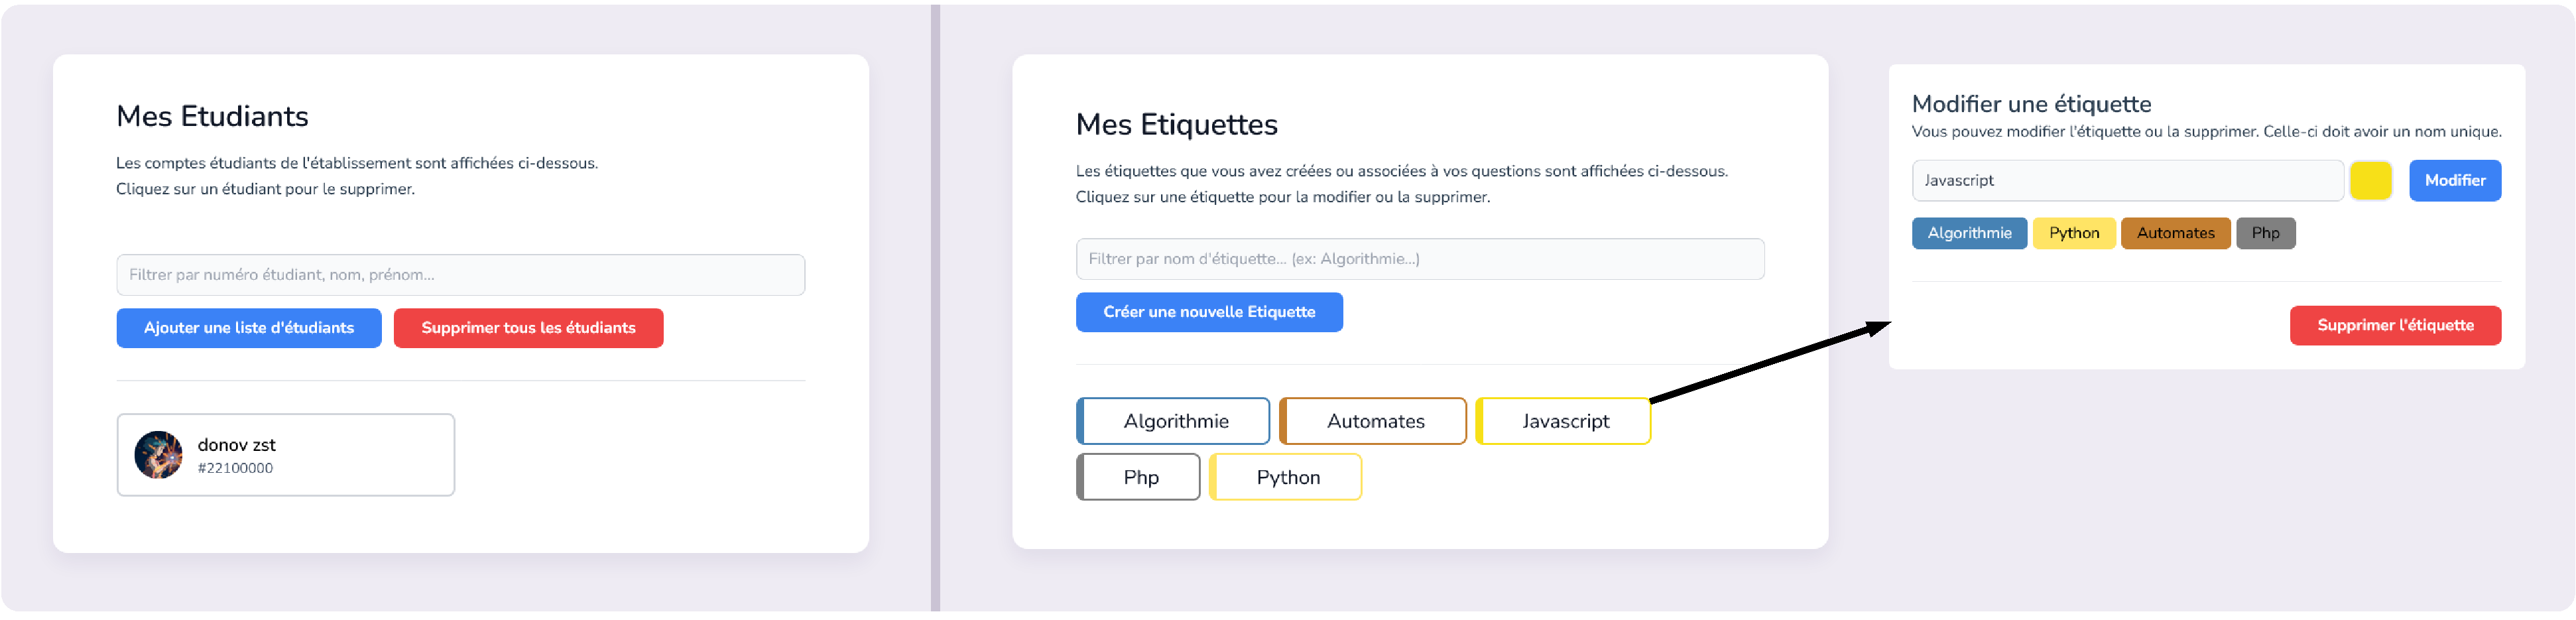
\includegraphics[width=\textwidth]{Ajouts.pdf}
\caption{Pages "Mes Etudiants" et "Mes étiquettes"}
\label{fig:ajouts}
\centering
\end{figure}
\vspace{3mm}

Nous avons aussi ajouté la possibilité, pour les étudiants, de personnaliser leur profil. Ils peuvent désormais modifier leur image de profil. Cette dernière est visible par les enseignants dans la page de gestion des utilisateurs et dans la page des statistiques. La couleur du profil, comme le montre la figure \ref{fig:profil}, est déterminée par la couleur prédominante de l'image de profil.\\

\vspace{2mm}
\begin{figure}[H]
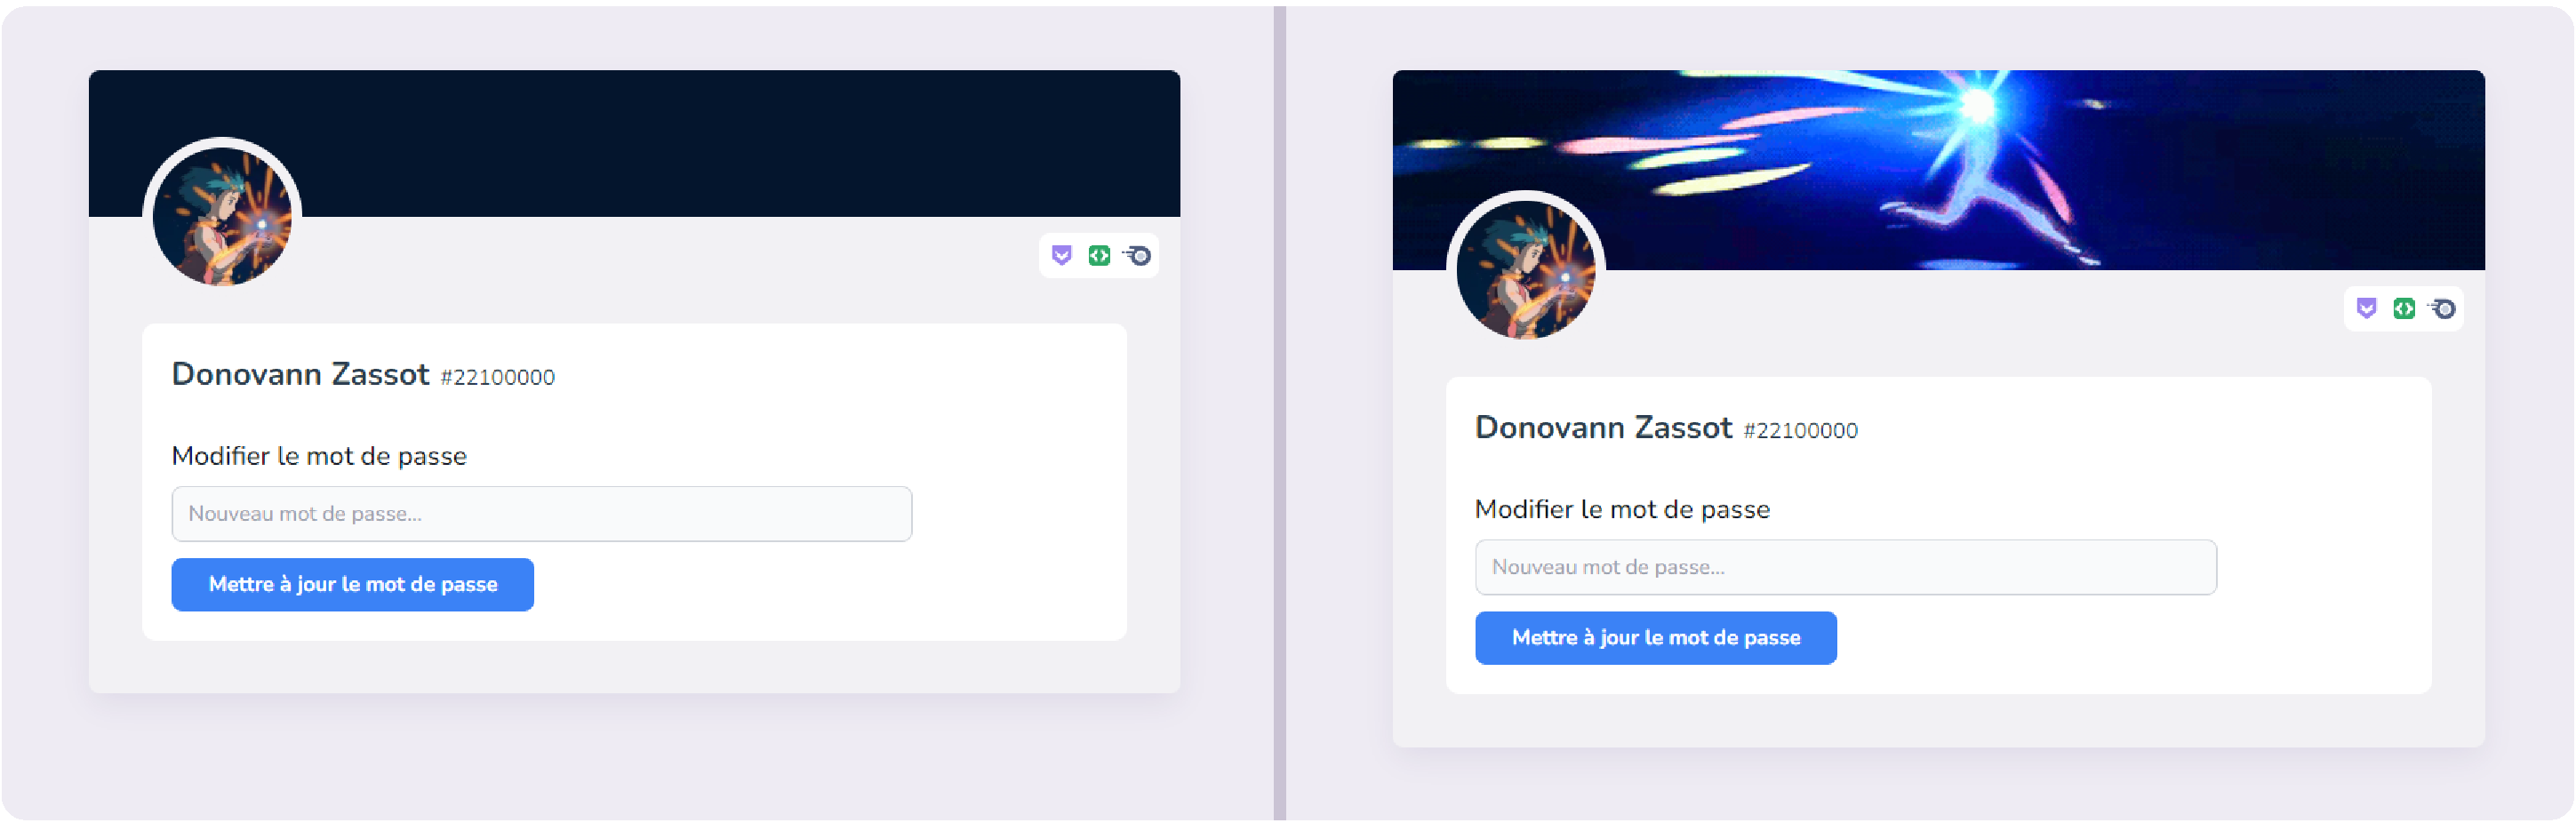
\includegraphics[width=\textwidth]{Profil.pdf}
\caption{Pages de Profil Etudiant (et la version de la page avec l'easter-egg activé)}
\label{fig:profil}
\centering
\end{figure}
\newpage

Enfin, pour rendre l'expérience utilisateur plus agréable, nous avons inclus plusieurs références et easter-eggs dans notre application. Parmi ceux-ci, vous trouverez :\\

\begin{itemize}
\setlength\itemsep{1em}
\item[•] La page de profil étudiant est une référence à l'interface utilisateur de Discord. En effet, nous avons, sur cette page uniquement, repris les éléments de design de Discord. Grâce à cela nous souhaitons créer une expérience familière pour les utilisateurs étudiants de notre site.

\item[•] Dans la page de profil étudiant, nous avons choisi les badges Discord. Le premier est une référence à la hypesquad de Discord avec le choix de la maison Bravery pour représenter l'équipe de développement\footnotemark[1], le second est le badge \textit{Developpeur Actif} et le troisième, le badge \textit{Nitro}.

\item[•] En cliquant sur un de ces badges, l'utilisateur débloque la possibilité de modifier le fond du profil étudiant comme avec Discord Nitro (côté client uniquement). Il peut alors choisir un fichier image qui sera défini comme fond. L'image peut être animée (gif). Vous pouvez avoir un aperçu du rendu dans la figure \ref{fig:ajouts}.

\item[•] La page d'accueil "Mes dernières Séquences" contient également un easter-egg. En cliquant sur le mot "champ", un carrousel apparaît. Celui-ci contient 5 images contenant des jeux de mots avec "champ". 

\item[•] Lorsqu'un étudiant rejoint une diffusion, il arrive sur une page d'attente. S'il le souhaite, il peut cliquer sur le mot "patience" pour jouer au Memory avec les mascottes du jeu (Bubule, Marinette ou Octave). Le jeu de mémory a été développé spécialement pour le projet, 7 listes de cartes sont disponibles et jouables aléatoirement. Le jeu montre aussi le nombre de tours joués et meilleur score qui est enregistré en local storage. La partie se termine automatiquement dès que la diffusion commence.
\end{itemize}

\vspace{3mm}
\begin{figure}[H]
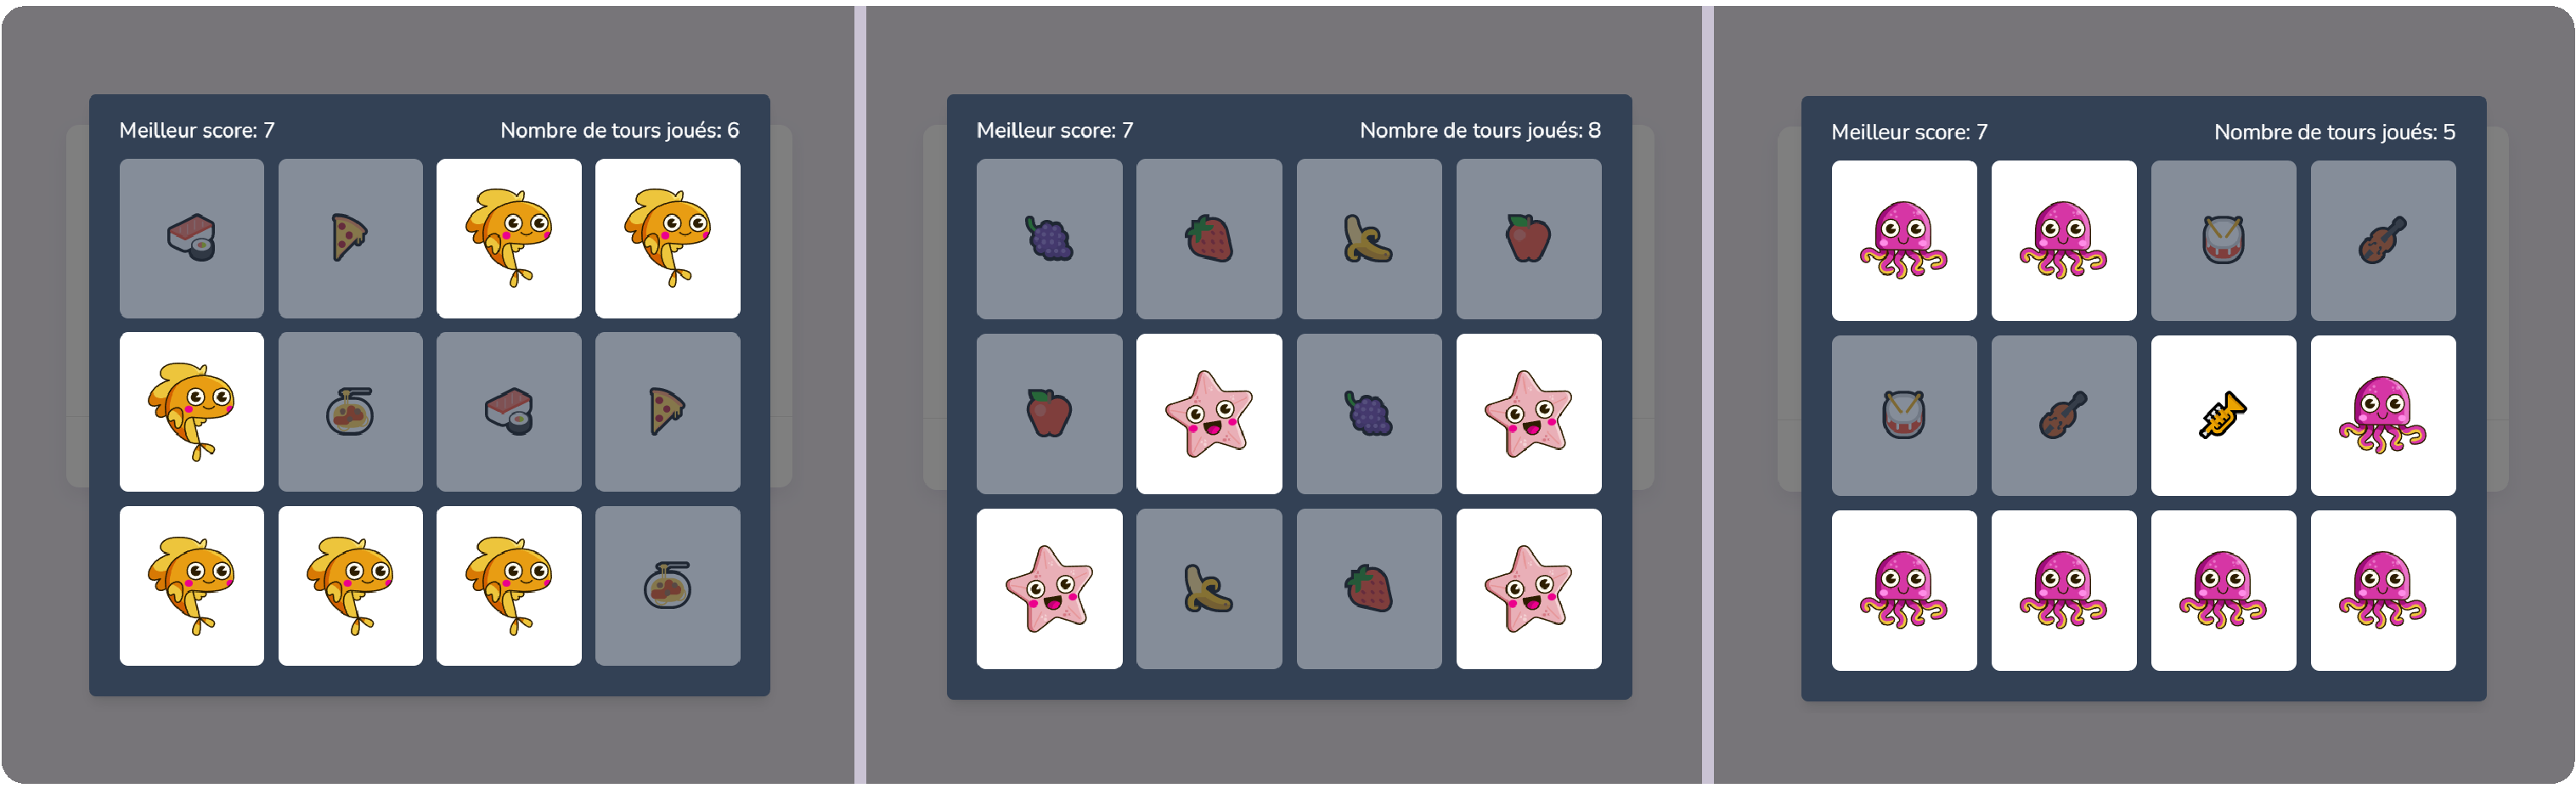
\includegraphics[width=\textwidth]{Memory.pdf}
\caption{Jeu de mémory avec les mascottes: un petit moment ludique !}
\label{fig:memory}
\centering
\end{figure}

\footnotetext[1]{Les quatre membres de l'équipe de développement font partie de la maison Bravery. Les maisons de la Hypesquad sont similaires aux maisons de Poudlard dans la série Harry Potter, où chaque maison représente une certaine qualité et des valeurs spécifiques. }